\documentclass[11pt,a4paper]{article}

\usepackage{amsmath} %for mathemathic formulas
\usepackage{amssymb}
\usepackage[ngerman]{babel} %for the german language by the spellling reform (without the package the date would look like April 20, 2020)
\usepackage{enumitem} %for enumeration surrounding
\usepackage{graphicx} %for pictures
\usepackage{siunitx}

\title{Blatt 6}
\date{\today}
\author{Hannah Rotgeri \and Lena Olbrich}

\begin{document}
    \maketitle

    \section*{Aufgabe 12}
\subsection*{Aufgabenteil a}
Population 0: (1;1) (2;1) (1,5; 2) (2;2) (2;3) (3;3) \\
Population 1: (1.5; 1) (2.5; 1) (3.5; 1) (2.5; 2) (3.5; 2) (4.5; 2)
\\
\noindent a)  Berechnen Sie die Mittelwerte 𝜇⃗und Streumatrizen 𝑆𝑖, sowie die kombinierte Streumatrix 𝑆𝑖𝑗.

\noindent \textbf{Mittelwerte}:
$\vec{\mu}=
\begin{pmatrix}
\bar{x} \\
\bar{y}
\end{pmatrix}=
\frac{1}{N}\begin{pmatrix}
\sum_{i=1}^{N} x_{i} \\
\sum_{i=1}^{N} y_{i}
\end{pmatrix}
$ \\
$
\rightarrow \vec{\mu_0}=
\begin{pmatrix}
\frac{23}{12} \\
2
\end{pmatrix},
\vec{\mu_1}=
\begin{pmatrix}
3 \\
\frac{3}{2}
\end{pmatrix}
$

\noindent \textbf{Streumatrix}:
$
S_i = \sum_{j=1}^{N_i} (\vec{x}_{j}-\vec{\mu}_{j})(\vec{x}_{j}-\vec{\mu}_{j})^T \\
S_0=
\begin{pmatrix}
-\frac{11}{12}\\
-1
\end{pmatrix} \begin{pmatrix}
-\frac{11}{12}\\
-1
\end{pmatrix}^T
+\begin{pmatrix}
\frac{1}{12}\\
-1
\end{pmatrix}\begin{pmatrix}
\frac{1}{12}\\
-1
\end{pmatrix}^T +
\begin{pmatrix}
-\frac{5}{12}\\
0
\end{pmatrix}
\begin{pmatrix}
-\frac{5}{12}\\
0
\end{pmatrix}^T +
\begin{pmatrix}
\frac{1}{12}\\
0
\end{pmatrix}\begin{pmatrix}
\frac{1}{12}\\
0
\end{pmatrix}^T +
\begin{pmatrix}
\frac{1}{12}\\
1
\end{pmatrix}
\begin{pmatrix}
\frac{1}{12}\\
1
\end{pmatrix}^T +
\begin{pmatrix}
\frac{13}{12}\\
1
\end{pmatrix}\begin{pmatrix}
\frac{13}{12}\\
1
\end{pmatrix}^\top \\
=\begin{pmatrix}
\frac{121}{144} & \frac{11}{12} \\
\frac{11}{12} & 1
\end{pmatrix} +
\begin{pmatrix}
\frac{1}{144} & \frac{-1}{12} \\
-\frac{1}{12} & 1
\end{pmatrix}+
\begin{pmatrix}
\frac{25}{144} & 0 \\
0 & 0
\end{pmatrix} +
\begin{pmatrix}
\frac{1}{144} & 0 \\
0 & 0
\end{pmatrix}+
\begin{pmatrix}
\frac{1}{144} & \frac{1}{12} \\
\frac{1}{12} & 1
\end{pmatrix}+
\begin{pmatrix}
\frac{169}{144} & \frac{13}{12} \\
\frac{13}{12} & 1
\end{pmatrix} =
\begin{pmatrix}
\frac{53}{24} & 2 \\
2 & 4

\end{pmatrix}
$
\\
$
S_1= \begin{pmatrix}
\frac{9}{4} & \frac{3}{4} \\
\frac{3}{4} & \frac{1}{4}
\end{pmatrix} +
\begin{pmatrix}
\frac{1}{4} & \frac{1}{4} \\
\frac{1}{4} & \frac{1}{4}
\end{pmatrix}+
\begin{pmatrix}
\frac{1}{4} & -\frac{1}{4} \\
-\frac{1}{4} & \frac{1}{4}
\end{pmatrix}+
\begin{pmatrix}
\frac{1}{4} & -\frac{1}{4} \\
-\frac{1}{4} & \frac{1}{4}
\end{pmatrix}+
\begin{pmatrix}
\frac{1}{4} & \frac{1}{4} \\
\frac{1}{4} & \frac{1}{4}
\end{pmatrix}+
\begin{pmatrix}
\frac{9}{4} & \frac{3}{4} \\
\frac{3}{4} & \frac{1}{4}
\end{pmatrix} \\=
\begin{pmatrix}
\frac{11}{2} & \frac{3}{2} \\
\frac{3}{2} & \frac{13}{2}
\end{pmatrix}
$

\noindent \textbf{Gesamtstreuung:} $S_W =
\sum_i^{N} S_i = S_0 + S_1 $
\rightarrow $S_W = \begin{pmatrix}
\frac{185}{24} & \frac{7}{2} \\
\frac{7}{2} & \frac{11}{2}
\end{pmatrix}
$
\subsection*{Aufgabenteil b}
(b) Wie lautet $\vec{\lambda}$?

\noindent $ \vec{\lambda}=
S_W^{-1}(\vec{\mu}_0-\vec{\mu}_1)
$
Mit $
S_W^{-1}= \frac{1}{Det S_W} \begin{pmatrix}
\frac{11}{2} & -\frac{7}{2} \\
-\frac{7}{2} & \frac{185}{24}
\end{pmatrix}= \frac{48}{1447}\begin{pmatrix}
\frac{11}{2} & -\frac{7}{2} \\
-\frac{7}{2} & \frac{185}{24}
\end{pmatrix} =\begin{pmatrix}
0,182 & -0,116 \\
-0,116 & 0,256
\end{pmatrix}
$
\rightarrow
$ \vec{\lambda} = \begin{pmatrix}
-0,256  \\
0,254
\end{pmatrix}
$ \\
$\vec{\lambda}= \lambda \vec{e}_{\lambda} = 0,360
\begin{pmatrix}
-0,710  \\
0,704
\end{pmatrix}
$

\subsection*{Aufgabenteil c}
Zeichnen Sie die Punkte der beiden Populationen in einen Graphen ein, zusammen mit der Projektionsgeraden

\begin{figure}[h]

	\centering

	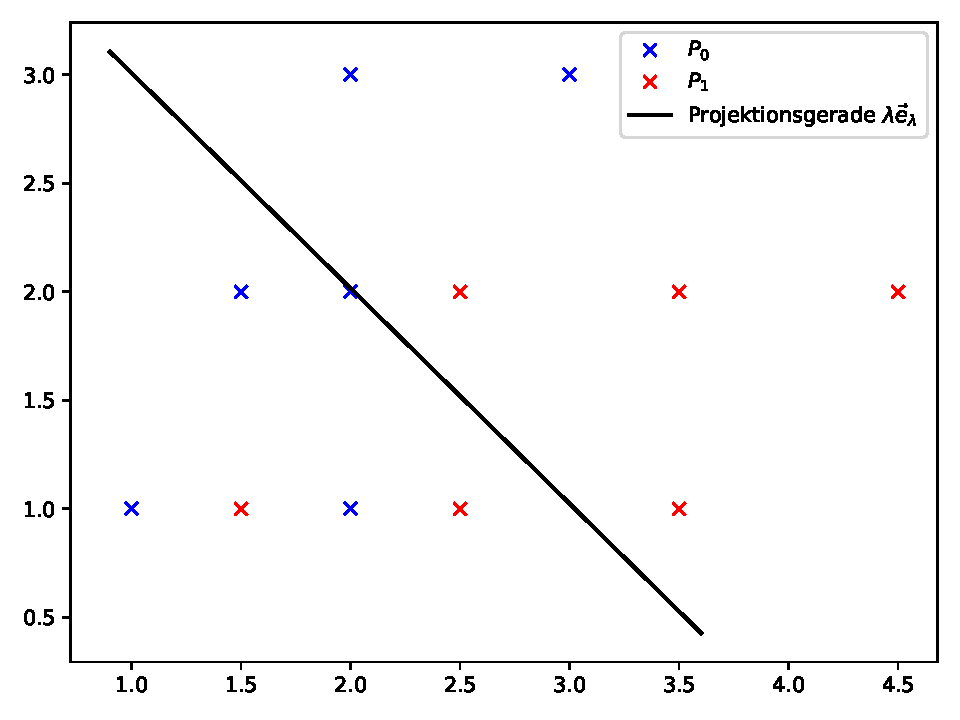
\includegraphics[width=\textwidth]{c.pdf}

	\caption{Ergebnis der Testdatei von Aufgabe 2}

\end{figure}

\subsection*{Aufgabenteil d}

Projektion= $\vec{\lambda}^T \cdot x$

Population 0: -0.006; -0.716; 0.343; -0.012; 0.693; -0.017
Population 1: -0.361; -1.071; -1.781; -0.367; -1.076; -1.786

\subsection*{Aufgabenteil e}
$\lambda_{cut}= -0.360$ sinnvoll, da hierbei 5/6 von Population 0 und 6/6 von Population 1 richtig zugeordnet werden.

\rightarrow
$t_p= 6, t_n=5,f_p= 1, f_n=0
$
\rightarrow Reinheit=$\frac{\text{tp}}{\text{tp + fp}}= \frac{6}{7}$ \\
Effizienz= $\frac{\text{tp}}{\text{tp + fn}}= \frac{6}{6}=1$
\end{document}
